% Figure for MATH 591 §76 (Lecture 30), generated by courses/591/new/2026-11-13-L30/gen.py
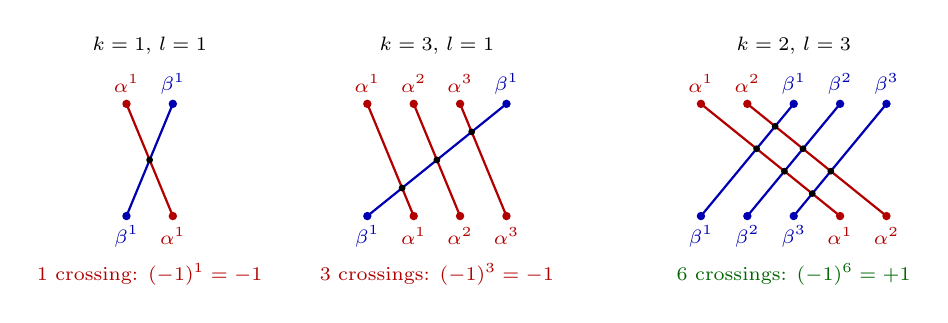
\begin{tikzpicture}[scale=0.95]
\draw[blue!70!black, thick] (0.620,1.500) -- (0.000,0.000);
\draw[red!70!black, thick] (0.000,1.500) -- (0.620,0.000);
\fill[black] (0.310,0.750) circle (1.3pt);
\fill[red!70!black] (0.000,1.500) circle (1.6pt);
\node[font=\scriptsize, text=red!70!black] at (0.000,1.770) {$\alpha^{1}$};
\fill[red!70!black] (0.620,0.000) circle (1.6pt);
\node[font=\scriptsize, text=red!70!black] at (0.620,-0.270) {$\alpha^{1}$};
\fill[blue!70!black] (0.620,1.500) circle (1.6pt);
\node[font=\scriptsize, text=blue!70!black] at (0.620,1.770) {$\beta^{1}$};
\fill[blue!70!black] (0.000,0.000) circle (1.6pt);
\node[font=\scriptsize, text=blue!70!black] at (0.000,-0.270) {$\beta^{1}$};
\node[font=\scriptsize] at (0.310,2.280) {$k = 1$, $l = 1$};
\node[font=\scriptsize, text=red!70!black] at (0.310,-0.780) {$1$ crossing: $(-1)^{1} = - 1$};
\draw[blue!70!black, thick] (5.080,1.500) -- (3.220,0.000);
\draw[red!70!black, thick] (3.220,1.500) -- (3.840,0.000);
\draw[red!70!black, thick] (3.840,1.500) -- (4.460,0.000);
\draw[red!70!black, thick] (4.460,1.500) -- (5.080,0.000);
\fill[black] (3.685,0.375) circle (1.3pt);
\fill[black] (4.150,0.750) circle (1.3pt);
\fill[black] (4.615,1.125) circle (1.3pt);
\fill[red!70!black] (3.220,1.500) circle (1.6pt);
\node[font=\scriptsize, text=red!70!black] at (3.220,1.770) {$\alpha^{1}$};
\fill[red!70!black] (3.840,0.000) circle (1.6pt);
\node[font=\scriptsize, text=red!70!black] at (3.840,-0.270) {$\alpha^{1}$};
\fill[red!70!black] (3.840,1.500) circle (1.6pt);
\node[font=\scriptsize, text=red!70!black] at (3.840,1.770) {$\alpha^{2}$};
\fill[red!70!black] (4.460,0.000) circle (1.6pt);
\node[font=\scriptsize, text=red!70!black] at (4.460,-0.270) {$\alpha^{2}$};
\fill[red!70!black] (4.460,1.500) circle (1.6pt);
\node[font=\scriptsize, text=red!70!black] at (4.460,1.770) {$\alpha^{3}$};
\fill[red!70!black] (5.080,0.000) circle (1.6pt);
\node[font=\scriptsize, text=red!70!black] at (5.080,-0.270) {$\alpha^{3}$};
\fill[blue!70!black] (5.080,1.500) circle (1.6pt);
\node[font=\scriptsize, text=blue!70!black] at (5.080,1.770) {$\beta^{1}$};
\fill[blue!70!black] (3.220,0.000) circle (1.6pt);
\node[font=\scriptsize, text=blue!70!black] at (3.220,-0.270) {$\beta^{1}$};
\node[font=\scriptsize] at (4.150,2.280) {$k = 3$, $l = 1$};
\node[font=\scriptsize, text=red!70!black] at (4.150,-0.780) {$3$ crossings: $(-1)^{3} = - 1$};
\draw[blue!70!black, thick] (8.920,1.500) -- (7.680,0.000);
\draw[blue!70!black, thick] (9.540,1.500) -- (8.300,0.000);
\draw[blue!70!black, thick] (10.160,1.500) -- (8.920,0.000);
\draw[red!70!black, thick] (7.680,1.500) -- (9.540,0.000);
\draw[red!70!black, thick] (8.300,1.500) -- (10.160,0.000);
\fill[black] (8.424,0.900) circle (1.3pt);
\fill[black] (8.796,0.600) circle (1.3pt);
\fill[black] (9.168,0.300) circle (1.3pt);
\fill[black] (8.672,1.200) circle (1.3pt);
\fill[black] (9.044,0.900) circle (1.3pt);
\fill[black] (9.416,0.600) circle (1.3pt);
\fill[red!70!black] (7.680,1.500) circle (1.6pt);
\node[font=\scriptsize, text=red!70!black] at (7.680,1.770) {$\alpha^{1}$};
\fill[red!70!black] (9.540,0.000) circle (1.6pt);
\node[font=\scriptsize, text=red!70!black] at (9.540,-0.270) {$\alpha^{1}$};
\fill[red!70!black] (8.300,1.500) circle (1.6pt);
\node[font=\scriptsize, text=red!70!black] at (8.300,1.770) {$\alpha^{2}$};
\fill[red!70!black] (10.160,0.000) circle (1.6pt);
\node[font=\scriptsize, text=red!70!black] at (10.160,-0.270) {$\alpha^{2}$};
\fill[blue!70!black] (8.920,1.500) circle (1.6pt);
\node[font=\scriptsize, text=blue!70!black] at (8.920,1.770) {$\beta^{1}$};
\fill[blue!70!black] (7.680,0.000) circle (1.6pt);
\node[font=\scriptsize, text=blue!70!black] at (7.680,-0.270) {$\beta^{1}$};
\fill[blue!70!black] (9.540,1.500) circle (1.6pt);
\node[font=\scriptsize, text=blue!70!black] at (9.540,1.770) {$\beta^{2}$};
\fill[blue!70!black] (8.300,0.000) circle (1.6pt);
\node[font=\scriptsize, text=blue!70!black] at (8.300,-0.270) {$\beta^{2}$};
\fill[blue!70!black] (10.160,1.500) circle (1.6pt);
\node[font=\scriptsize, text=blue!70!black] at (10.160,1.770) {$\beta^{3}$};
\fill[blue!70!black] (8.920,0.000) circle (1.6pt);
\node[font=\scriptsize, text=blue!70!black] at (8.920,-0.270) {$\beta^{3}$};
\node[font=\scriptsize] at (8.920,2.280) {$k = 2$, $l = 3$};
\node[font=\scriptsize, text=green!40!black] at (8.920,-0.780) {$6$ crossings: $(-1)^{6} = + 1$};
\end{tikzpicture}
